\documentclass[conference]{IEEEtran}
\IEEEoverridecommandlockouts

\usepackage{cite}
\usepackage{amsmath,amssymb,amsfonts}
\usepackage{algorithmic}
\usepackage{graphicx}
\usepackage{textcomp}
\usepackage{xcolor}
\usepackage[hyphens]{url}
\usepackage{hyperref}
\hypersetup{colorlinks=true,allcolors=black}
\newcommand{\srclink}[2]{\href{#1}{\underline{#2}}}
\newcommand{\repo}{https://github.com/FudanSELab/train-ticket/blob/813dd01/}
\newcommand{\src}[2]{\href{\repo#1}{\nolinkurl{#2}}}
\usepackage{booktabs}
\usepackage{tabularx}
\usepackage{array}

\begin{document}

\title{CC4M: Code Clone Analysis and Visualization for Microservices}

\author{
\IEEEauthorblockN{Gen Kawamata, Yuki Ota, Norihiro Yoshida, Shiyu Yang, Erina Makihara, Katsuro Inoue}
\IEEEauthorblockA{
Ritsumeikan University\\
Osaka, Japan\\
\{is0665sp, is0607ih\}@ed.ritsumei.ac.jp,
\{norihiro, yangsy, makihara, inoue-k\}@fc.ritsumei.ac.jp
}
}

\maketitle

\begin{abstract}
Microservice architecture supports software evolution by 
decomposing a system into small, loosely coupled services 
that can be deployed independently.
Contrary to the expectation of high modularity, prior studies have reported that code clones exist across service boundaries, some of which are co-modified in the same version.
Such clones may require changes to be propagated across service boundaries, 
thereby undermining service independence and increasing maintenance costs.
However, existing tools do not support microservice-aware clone analysis.
We present CC4M, a microservice-aware clone analysis and visualization
tool. 
CC4M detects and enriches clone pairs with service-boundary, co-modification, file-category, and metric information. The enriched clones are visualized in an interactive scatter plot with explicit service boundaries, supporting metric-based filtering to prioritize clones with potentially higher maintenance impact.
Using an open-source microservice application, we illustrate how CC4M
helps identify the potential impact scope of code changes. 
A demo video and the tool are available at https://www.youtube.com/watch?v=0xOIQPFbkUg and https://github.com/gg117e/CC4M, respectively.

% Moの研究では，same versionとの記述
% 2/3くらいまで減らす（背景を減らしてもいいかも）
% file カテゴリに統一


% マイクロサービスアーキテクチャは，システムを小規模で疎結合かつ
% 独立してデプロイ可能なサービス群へ分割することで，ソフトウェア進化を支援する．
% しかし，先行研究では，マイクロサービスシステムにおいて
% サービス間コードクローンが存在し，その一部が同一コミット内で同時修正されていることが
% 報告されている．このようなクローンは，サービス境界を越えて変更を波及させる可能性があり，
% サービスの独立性を損ない，保守コストを増加させる要因となる．
% 本稿では, マイクロサービスシステムを対象としたコードクローン検出, 可視化ツール
% である CC4M を提案する. CC4M は Type-2 クローンペアを検出し,
% それらにサービス境界, 同時修正, およびファイルカテゴリの情報を付与した上で,
% service span や co-modification frequency などのクローンメトリクスを計算する.
% 拡張されたクローンは, 明示的なサービス境界を持つインタラクティブな散布図として
% 可視化され, CC4M はメトリクスに基づくフィルタリングにより, 保守上の影響が
% 大きいクローンの優先付けを支援する.
% あるオープンソースのマイクロサービスアプリケーションを用いて, コード変更の潜在的な
% 影響範囲の特定やリファクタリング候補の発見など, CC4M がソフトウェア進化タスクを
% どのように支援するかを示す.
% デモ動画は [URL] で公開する.

\end{abstract}

\begin{IEEEkeywords}
microservices, code clone, visualization
\end{IEEEkeywords}


\section{Introduction}

Microservice architecture decomposes a software system into small, loosely
coupled, and independently deployable services. It has been widely adopted
in both open-source and industrial projects, including systems at Netflix,
Amazon, and Spotify, to support software evolution through modularity and
technology heterogeneity
\cite{Richardson2018MicroservicesPatterns,Newman2021BuildingMicroservices,LewisFowler2014Microservices}.
% In a microservice system, each service may be implemented using different
% technologies and is expected to evolve independently.

Because microservices emphasize modularity and service independence, one might expect clones across service boundaries to be limited. 
% Code clones
% are code fragments that are identical or similar to one
% another~\cite{RoyCordy2009}. 
% Such pairs and sets of similar fragments are called clone pairs and clone sets, respectively.
However, Mo et al. reported that code clones exist across
microservices in open-source microservice projects, and showed that
clones are co-modified across service boundaries between consecutive releases~\cite{Mo2021ESEM}.
% 追加
Here, code clones are identical or similar code fragments~\cite{RoyCordy2009}; a clone pair is a pair of such fragments, and a clone set is a set of mutually similar fragments.
Co-modification refers to the case in which the code fragments
constituting a clone pair are modified together in the project's revision history.
% versionの表現を修正
Following prior work~\cite{Mo2021ESEM}, we classify clone
pairs in microservice systems based on service boundaries. 
A clone pair is called a \emph{within-service clone pair} when both fragments belong to the same service, and a \emph{cross-service clone pair} when the two fragments belong to different services~\cite{Mo2021ESEM}.
% サービス内・間クローンの定義を変更
% A clone pair
% is regarded as a within-service clone when both fragments belong to the
% same service, and as a cross-service clone when the fragments belong to
% different services. 
In subsequent work, Zhao et al. analyzed cross-service
clones based on file categories and showed that the distribution and
underlying causes of clones differ across categories~\cite{Zhao2022ICPC}.
% 削減
% Co-modifications of cross-service clones are important from a software
% evolution perspective because they suggest that changes to a cloned
% fragment in one service may require consistent changes to its cloned
% fragments in other services. Such cross-service change coupling can
% undermine service independence and make maintenance more
% difficult~\cite{Mo2021ESEM,Zhao2022ICPC}.
%
% Existing clone detection and visualization tools
% \cite{Ueda2002Gemini,Asaduzzaman2011VisCad,Voinea2014SolidSDD}
% support the inspection of clone detection results, but they are not
% designed for microservice-specific analysis. In particular, they lack
% two capabilities: (i) service-boundary awareness, so within-service and
% cross-service clones are not distinguished and the scope of change
% impact is unclear; and (ii) co-modification awareness, so historical
% change coupling is not integrated, hindering the identification of
% clones that affect maintainability.

These findings indicate that cross-service clones exist, are co-modified, and concentrate in specific file categories, suggesting that such clones may propagate changes across service boundaries and undermine service independence. However, existing clone detection and visualization tools~\cite{Ueda2002Gemini,Asaduzzaman2011VisCad,Voinea2014SolidSDD} organize clone information by file system or program structure (e.g., directories, files, and classes) rather than by service boundaries. In particular, they lack two capabilities: (i) service-boundary awareness, so within-service and cross-service clone pairs are not distinguished and the scope of change impact is unclear; and (ii) co-modification awareness, so historical change coupling is not integrated, hindering the identification of clones that affect maintainability.

To address these limitations, we introduce \textsc{CC4M},
a tool for detecting and
visualizing code clones in microservice systems. It detects Type-2
clones with CCFinderSW, a code clone detector that supports multiple
programming languages~\cite{Semura2017CCFinderSW}, and identifies service
boundaries with CLAIM~\cite{Maggi2024CLAIM}. 
\textsc{CC4M} then enriches each clone pair with service boundary, co-modification, and file-category information, the last of which is inspired by the file-level analysis of Zhao et al. \cite{Zhao2022ICPC}.
% 3つのビューを紹介
Based on the enriched information, \textsc{CC4M} computes clone metrics,
such as service span and co-modification
frequency. The enriched clone pairs are visualized through three views:
a \emph{Statistics View} that summarizes project-wide clone statistics,
an interactive \emph{Scatter Plot} with explicit service boundaries,
and a \emph{Metric View} for metric-based prioritization and
drill-down across services, clone sets, and files.

The contributions of this paper are as follows.
First, we present \textsc{CC4M}, a microservice-aware clone analysis tool
that enriches clone pairs with service-boundary, co-modification,
and file-category information.
Second, we introduce clone metrics, such as service span and
co-modification frequency, to quantify the impact scope and change
coupling across service boundaries.
Third, we provide a scatter plot with explicit service boundaries and
a \emph{Metric View} for metric-based prioritization and drill-down.


\section{CC4M}
\label{sec:CC4M}

\begin{figure*}[tb]
\centering
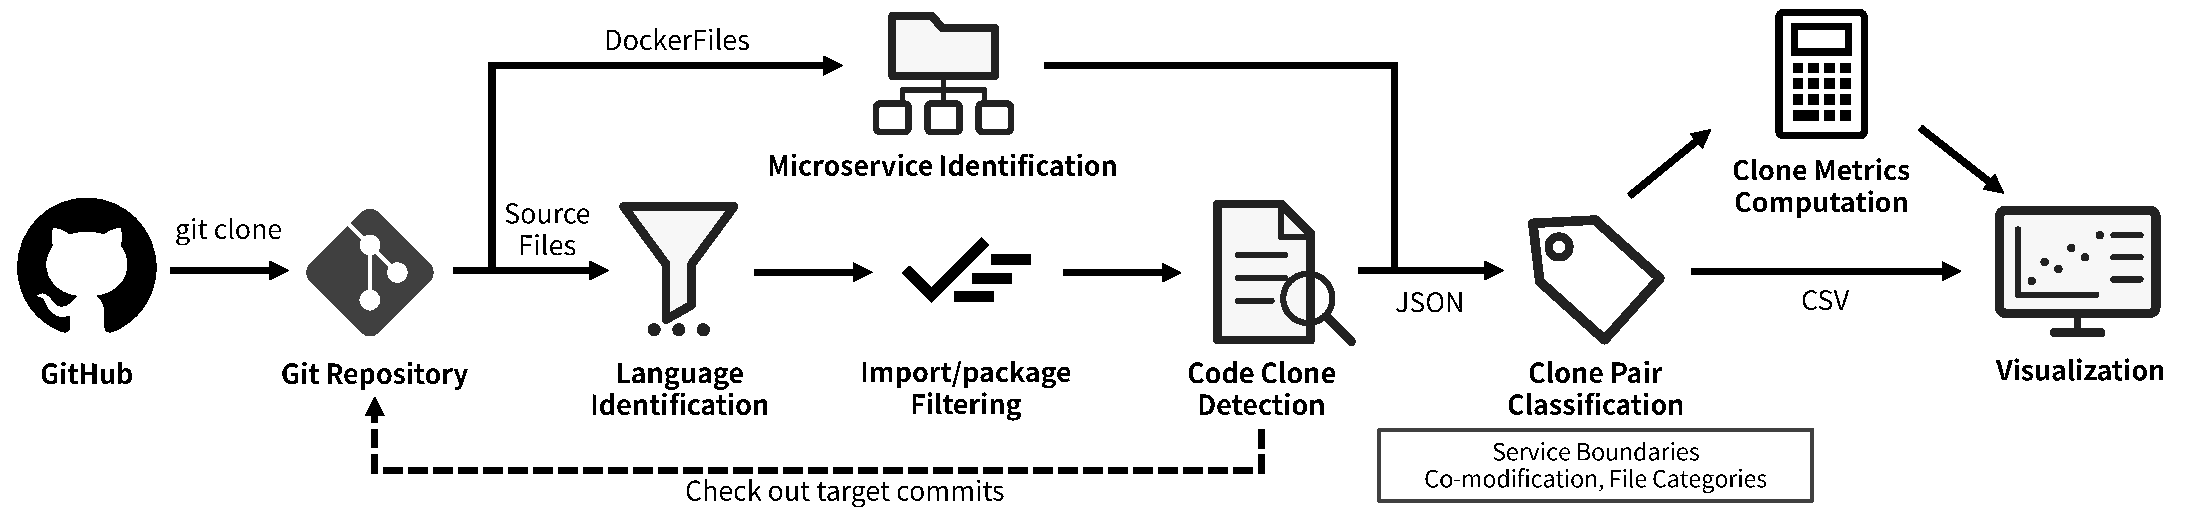
\includegraphics[width=1.0\linewidth]{img/overview.pdf}
\caption{
An overview of \textsc{CC4M}. It identifies microservices from a Git repository, detects code clones,
enriches them with service boundaries, co-modification history, and file categories, computes clone metrics, and visualizes the results.
}
\label{fig:overview}
\end{figure*}


Fig.~\ref{fig:overview} shows an overview of \textsc{CC4M}. It takes as
input the GitHub URL of a Dockerized microservice system and provides
three views for exploring code clones: a \emph{Statistics View}, a \emph{Scatter
Plot}, and a \emph{Metric View}. To support these views, \textsc{CC4M} identifies
microservice boundaries, detects Type-2 clone pairs, and enriches them
with co-modification history and file-category information.
% CC4Mも斜体
% Hereafter,(MS-Base)



% Figure~\ref{fig:overview} は，CC4M の概要を示している．
% CC4M の入力は，Docker 化されたマイクロサービスシステムの GitHub URL であり,
% コードクローンを分析するための 3 つのビュー,
% すなわち Statistics View, Scatter Plot, および Metric View を提供する.
% これらのビューを支えるため, CC4M は, マイクロサービス境界を識別し,
% Type-2 クローンペアを検出し, それらに同時修正履歴とファイルカテゴリ情報を
% 付与する.


\subsection{Microservice Identification}
\label{sec:service_identification}

\textsc{CC4M} identifies microservices by applying CLAIM~\cite{Maggi2024CLAIM},
a lightweight static analysis approach based on Docker Compose files
and related Dockerfiles. CLAIM extracts service definitions from the
Docker configuration files and estimates which directories correspond to application microservices.
% 

\textsc{CC4M} then assigns each source file to a microservice based on the
directory information obtained by CLAIM. This assignment is used to
determine whether each clone pair is a within-service clone or a
cross-service clone.

% CC4M は，Docker Compose ファイルおよび関連する Dockerfile に基づく
% 軽量な静的解析手法である CLAIM~\cite{Maggi2024CLAIM} を用いて，
% マイクロサービスを識別する．CLAIM は Docker の構成ファイルから
% サービス定義を抽出し，アプリケーションのマイクロサービスに対応する
% ディレクトリを推定する．
%
% その後，CC4M は CLAIM によって得られたディレクトリ情報に基づいて，
% 各ソースファイルをマイクロサービスへ対応付ける．この対応関係は，
% 各クローンペアがサービス内クローンであるか，サービス間クローンであるかを
% 判定するために用いられる．


\subsection{Code Clone Detection}
\label{sec:clone_detection}

\textsc{CC4M} identifies the programming languages used in the target
repository using GitHub Linguist\footnote{\url{https://github.com/github-linguist/linguist}}
and selects source files whose languages are supported by CCFinderSW.

Before running CCFinderSW, \textsc{CC4M} comments out import, include,
and package declarations in a temporary analysis copy to exclude them
from the token sequence used for clone detection and reduce trivial clones.
The full list of filtered patterns is documented in our GitHub repository.\footnote{\url{https://github.com/gg117e/CC4M/blob/main/docs/declaration_filtering.md}}

\textsc{CC4M} then uses CCFinderSW~\cite{Semura2017CCFinderSW} to obtain
Type-2 clone pairs. Type-2 clones are clone pairs whose fragments are
identical except for differences in whitespace, comments, and identifiers
such as variable names and type names~\cite{RoyCordy2009}.
CCFinderSW supports multiple programming languages through ANTLR grammar
definitions, which makes it suitable for heterogeneous microservice
repositories.

% 削減
% The clone detection results produced by CCFinderSW are converted
% into JSON format using ccfindersw-parser\footnote{\url{https://github.com/YukiOhta0519/ccfindersw-parser}}
% and used as input for the subsequent co-modification analysis and
% clone pair classification.

% CC4M は，GitHub Linguist\footnote{\url{https://github.com/github-linguist/linguist}}
% を用いて対象リポジトリで使用されているプログラミング言語を識別し，
% CCFinderSW が対応する言語のソースファイルを分析対象として選択する．

% CCFinderSW を実行する前に，CC4M は一時的な分析用コピー上で
% import 文，include 文，および package 宣言をコメントアウトすることで，
% それらをクローン検出に用いるトークン列から除外し，自明なクローンを削減する．
% フィルタ対象パターンの一覧は GitHub リポジトリに記載されている\footnote{\url{https://github.com/gg117e/CC4M/blob/main/docs/declaration_line_filtering.md}}．

% 次に，CC4M は CCFinderSW~\cite{Semura2017CCFinderSW} を用いて
% Type-2 クローンペアを取得する．Type-2 クローンとは，空白，コメント，
% および変数名や型名などの識別子の違いを除いて一致するコード片からなる
% クローンペアである~\cite{RoyCordy2009}．
% CCFinderSW は ANTLR の文法定義を通じて複数のプログラミング言語に対応しており，
% 異種言語を含むマイクロサービスリポジトリの分析に適している．

% CCFinderSW によって生成されたクローン検出結果は，
% ccfindersw-parser\footnote{\url{https://github.com/YukiOhta0519/ccfindersw-parser}}
% を用いて JSON 形式に変換され，後続の同時修正分析およびクローンペア分類の入力として用いられる．

\subsection{Co-modification Analysis}
\label{sec:comodification}

\textsc{CC4M} identifies clone pairs that were modified together based on
Git history.
Users can select commits at a specified interval, merge commits, or
commits associated with Git tags, depending on the desired analysis
granularity.

For each selected target commit, \textsc{CC4M} performs clone detection and
tracks code fragments across adjacent target commits using line
correspondences obtained from \texttt{git diff}. For a tracked fragment,
\textsc{CC4M} regards it as modified at commit $c_i$ when lines in its
corresponding range are added, deleted, or changed between $c_{i-1}$
and $c_i$.

% コミット集合Cの定義をする
Let $A$ and $B$ be the two fragments forming a clone pair, and let
$C_A$ and $C_B$ be the sets of target commits in which $A$ and $B$ were
modified, respectively. \textsc{CC4M} regards the clone pair as co-modified
when $C_A \cap C_B \neq \emptyset$, that is, when both fragments were
modified in the same commit at least once.

% CC4M は，Git の変更履歴に基づいて，同時に修正されたクローンペアを特定する．
% 利用者は，分析粒度に応じて，一定間隔のコミット，マージコミット，
% または Git タグに対応するコミットを選択できる．

% CC4M は，各対象コミットにおいてコードクローン検出を実行し，
% \texttt{git diff} から得られる行対応関係を用いて，
% 隣接する対象コミット間でコード片を追跡する．
% 追跡されたコード片について，$C_{i-1}$ から $C_i$ への変更において，
% 対応する範囲内の行が追加，削除，または変更された場合，
% CC4M はそのコード片がコミット $C_i$ において修正されたとみなす．

% クローンペアを構成する 2 つのコード片を $A$ および $B$ とし，
% それぞれが修正された対象コミットの集合を $C_A$ および $C_B$ とする．
% CC4M は，$C_A \cap C_B \neq \emptyset$ である場合，
% すなわち，両方のコード片が少なくとも一度，同一コミット内で修正された場合，
% そのクローンペアを同時修正されたものとみなす．


\subsection{Clone Pair Classification}
\label{sec:classification}

\textsc{CC4M} annotates each clone pair with three kinds of information:
service-boundary, co-modification, and file-category.
Using the service mapping computed in
Section~\ref{sec:service_identification}, it classifies each pair
as either a within-service clone or a cross-service clone. Using the
co-modification information computed in Section~\ref{sec:comodification},
it records whether the pair has been co-modified in the Git history.

It also classifies each file into one of four categories: \emph{Test},
\emph{Config}, \emph{Data}, or \emph{Logic}. This classification is based on path and
file-name patterns, and rules are applied in this priority order.
It then assigns a category to each clone pair from the categories
of the two files containing the cloned fragments. Clone pairs whose
two files share the same category are categorized as \emph{Test}, \emph{Config}, or
\emph{Data}; pairs involving both test and non-test files are categorized as
\emph{Mixed}; and the remaining pairs are categorized as \emph{Logic}. The full
classification rules are documented in our GitHub repository\footnote{\url{https://github.com/gg117e/CC4M/blob/main/docs/file_classification.md}}.

% 分類は，パスおよびファイル名のパターンに基づいて行う．
% 概要として，パスまたはファイル名がテストコードを示す場合は
% \textit{Test}，設定ファイルである場合，または設定に関連するディレクトリに
% 存在する場合は \textit{Config}，パスまたはファイル名がエンティティ，
% DTO，データスキーマを示す場合は \textit{Data}，
% それ以外の場合は \textit{Logic} として分類する．
% 複数の規則が 1 つのファイルに一致する場合，CC4M は
% \textit{Test}，\textit{Config}，\textit{Data}，
% \textit{Logic} の順に，最初に一致したカテゴリを割り当てる．
% クローンペアを構成する 2 つのファイルのカテゴリに基づいて，
% CC4M はクローンペアカテゴリを割り当てる．
% 両方のファイルが同じカテゴリに属する場合，そのペアは
% \textit{Test}，\textit{Config}，または \textit{Data}
% として分類される．
% 一方のファイルがテストファイルであり，もう一方が非テストカテゴリに
% 属する場合，そのペアは \textit{Mixed} として分類される．
% それ以外の場合，そのペアは \textit{Logic} として分類される．
% 完全な分類規則は GitHub リポジトリに記載されている\footnote{\url{https://github.com/gg117e/CC4M/blob/main/docs/file_classification.md}}．


\subsection{Clone Metrics Computation}
\label{sec:clone_metrics}

The enriched clone pairs produced in Sections~\ref{sec:service_identification} to \ref{sec:classification} carry rich attributes, making individual inspection impractical.
To enable metric-based prioritization and filtering of the enriched clone pairs, \textsc{CC4M} characterizes them with clone metrics.
% クローンがたくさんあるのでフィルタリングする
% 見るのが大変
% 

\textbf{\(\mathbf{MS}(s)\). }
This metric represents the set of microservices to which the code fragments in a given clone set \(s\) belong.
Let \(f \in s\) denote a code fragment in clone set \(s\), and let \(\mathrm{ms}(f)\) denote the microservice to which fragment \(f\) belongs. Then, \(\mathrm{MS}(s) = \{\, \mathrm{ms}(f) \mid f \in s \,\}\), and \(|\mathrm{MS}(s)|\) represents the number of microservices spanned by clone set \(s\).
A clone set \(s\) satisfying \(|\mathrm{MS}(s)| \geq 2\) is called a \emph{cross-service clone set}.

\textbf{\(\mathbf{CM}(s)\).}
This metric represents the set of co-modification commits for a given clone set \(s\).
A commit \(c\) is called a \emph{co-modification commit} of \(s\) if at least two fragments in \(s\) are modified in \(c\).
Then, \(\mathrm{CM}(s)\) is defined as:
\[
\mathrm{CM}(s) = \{\, c \mid \text{at least two fragments in } s \text{ are modified in } c \,\}.
\]
This extends the pair-level co-modification in Section~\ref{sec:comodification}: \(c \in \mathrm{CM}(s)\) exactly when at least one clone pair within \(s\) is co-modified at \(c\).
\(|\mathrm{CM}(s)|\) represents the number of co-modification commits of \(s\).
The co-modification fragment ratio of \(s\), denoted by \(\mathrm{cmr}(s)\), is defined as the fraction of fragments in \(s\) that are modified in at least one commit in \(\mathrm{CM}(s)\).

In the \emph{Scatter Plot} and \emph{Metric View} (see Section~\ref{sec:visualization}), \(|\mathrm{MS}(s)|\), \(|\mathrm{CM}(s)|\), and \(\mathrm{cmr}(s)\) are shown as \textit{service span}, \textit{co-modification frequency}, and \textit{co-modification fragment ratio}, respectively.
In addition to these clone-set-level metrics, \textsc{CC4M} computes per-service and per-file metrics to support filtering and inspection, such as the number of cross-service clone sets, the ratio of cloned lines to service size, and the number of services shared through clone sets.
The full definitions of these additional metrics are documented in our GitHub repository\footnote{\url{https://github.com/gg117e/CC4M/blob/main/docs/metrics.md}}.


\subsection{Visualization}
\label{sec:visualization}

\begin{figure}[tb]
\centering
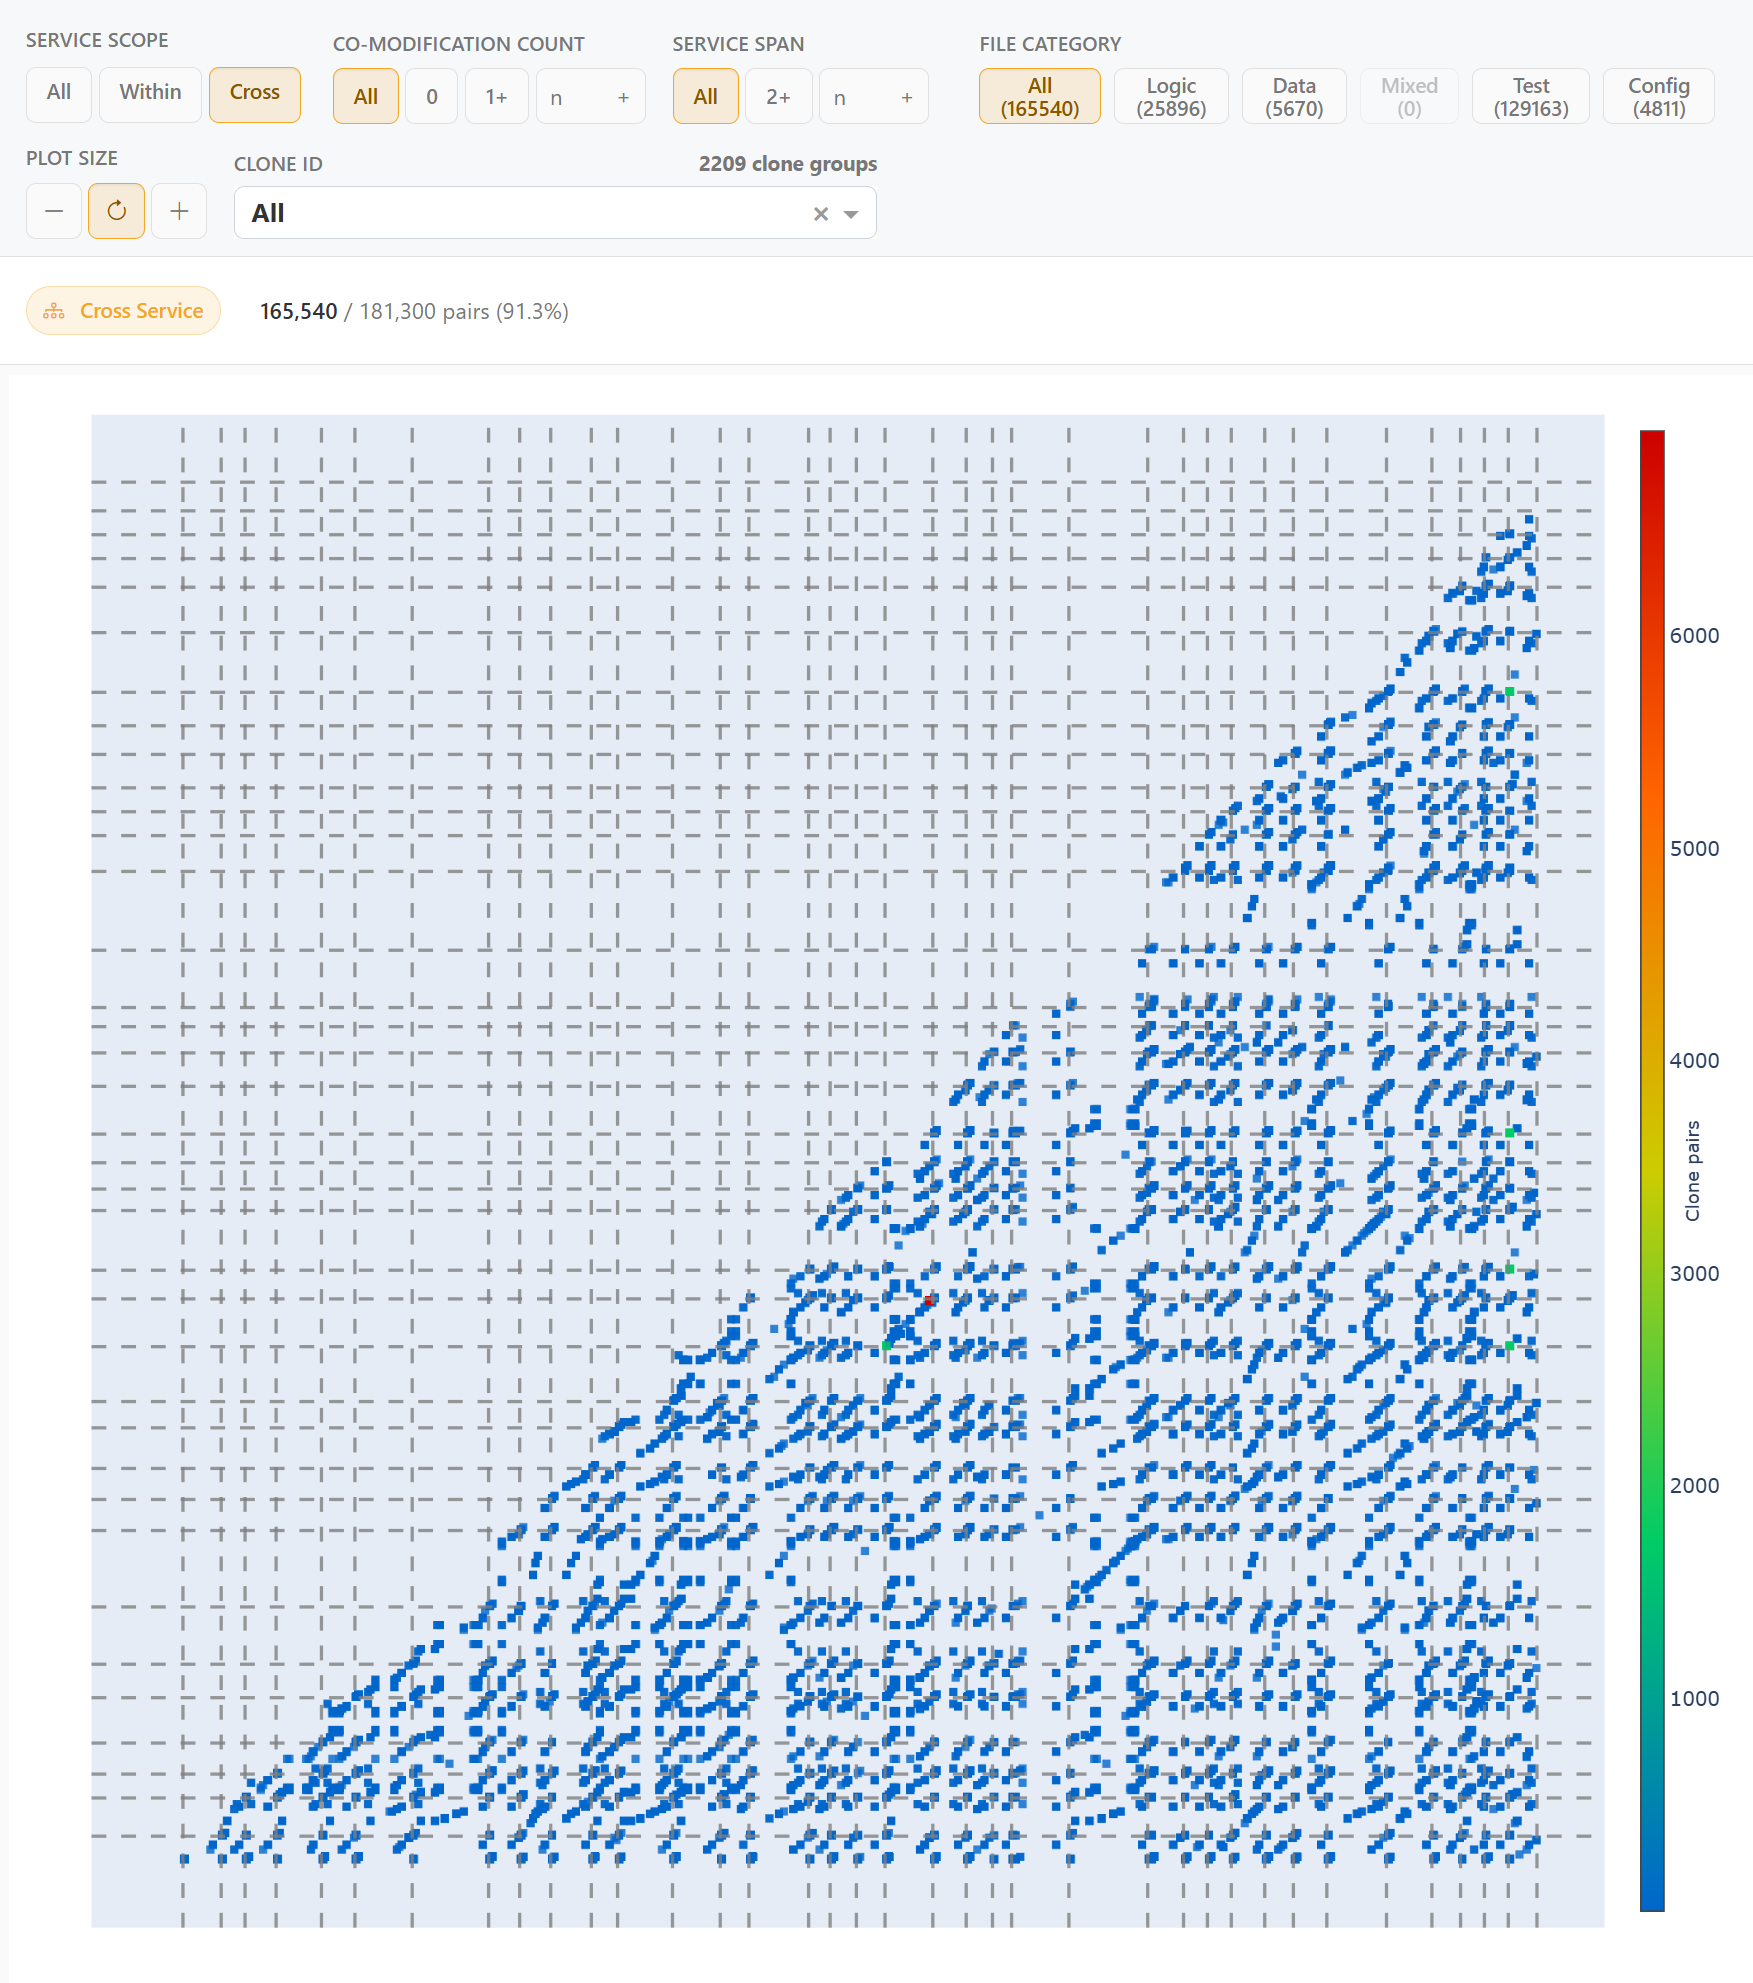
\includegraphics[width=1.0\linewidth]{img/scatter.png}
\caption{
A screenshot of the \textsc{CC4M} scatter plot generated for the \textsc{Train Ticket}
microservice project. The same source files are arranged on both axes
and grouped by microservice, with gray dotted lines indicating service
boundaries. The Service Scope filter is set to Cross, so the plot shows
only cross-service clone pairs. Each point represents clones between a
pair of files, and its color encodes the number of clone pairs.
}
\label{fig:scatter_view}
\end{figure}

\textsc{CC4M} provides three views: (i) a \emph{Statistics View} that reports
clone statistics for the entire project, (ii) a \emph{Scatter Plot} that visualizes
the spatial distribution of clone pairs across service boundaries,
and (iii) a \emph{Metric View} that supports metric-driven filtering
and drill-down across services, clone sets, and files.

\smallskip\noindent\textbf{Statistics View.}
It provides an overview of clones across the project. It summarizes the number of microservices, files, clone sets, and lines of code, breaks them down by language, and ranks the services that
concentrate the most clones.

\smallskip\noindent\textbf{Scatter Plot.}
Fig.~\ref{fig:scatter_view} shows a scatter plot in which the same set
of source files is arranged on both axes in the same order and grouped
by service. Gray dotted lines indicate service boundaries. A clone pair
is plotted at the coordinates of the two files containing the cloned
fragments; color intensity encodes overlapping clone pairs for the same
file pair. Points inside diagonal service blocks represent
within-service clones, whereas points outside represent cross-service
clones. This layout helps users locate clone concentrations across
services without inspecting individual file paths.
A filter panel lets users restrict the displayed clone pairs by service
scope, file category, and co-modification count. In
Fig.~\ref{fig:scatter_view}, Service Scope is set to Cross, so the plot
shows only cross-service clone pairs. Filters can also be combined; for
example, restricting file-category to Logic and Co-modification Count to
at least 1 surfaces cross-service Logic clones that have required
coordinated changes in the past. Users can zoom or pan to inspect dense
regions, and selecting a point opens a detail panel that shows the
corresponding cloned fragments with surrounding source code.
% Fig.に統一
% Code cloneはフラグメントのこと， Code fragment，

\smallskip\noindent\textbf{Metric View.}
It supports metric-based prioritization and drill-down
analysis of clone information. While the \emph{Scatter Plot} helps users
visually locate clone distributions across service boundaries, the
\emph{Metric View} helps users identify services, clone sets, and files that
are likely to have larger maintenance impact according to the computed
metrics.
% Merric View
The \emph{Metric View} provides three entry perspectives: Microservice-Based
(MS-Based), Clone-Set-Based, and File-Based. In each perspective, users
can narrow down the result list by combining multiple metric filters.
In Clone-Set-Based, users can focus on clone sets that span multiple
services or have past co-modifications by using metrics such as service
span and co-modification frequency. In MS-Based, users can identify
services that contain many cross-service clone sets or have a high
cloned-line ratio. In File-Based, users can find files that share clones
with many services or have cross-service co-modification histories.
The filtered results are shown as ranked lists, allowing users to
prioritize items before inspecting source code. When a clone set is
selected, the \emph{Metric View} displays the fragments contained in the
clone set. Users can then select one or two fragments to view the
corresponding source code. This staged workflow, from metric-based
prioritization to code-level inspection, helps users focus on clone
relationships that are more likely to affect maintenance tasks.


% CC4M は次の 3 種類のビューを提供する:
% (i) プロジェクト全体の統計を示す Statistics View,
% (ii) クローンの空間的分布を示す Scatter Plot,
% (iii) 複数メトリクスの組み合わせでクローンを絞り込む Metrics View.
%
% \textbf{Statistics View.}
% Statistics View は, プロジェクト全体のクローン分布を俯瞰するビューである.
% マイクロサービス数, ファイル数, クローンセット数, 総 LOC の集計値を言語別に
% 整理し, クローンが集中しているサービスをランキング表示する.
%
% \textbf{Scatter Plot.}
% Scatter Plot (Figure~\ref{fig:scatter_view}) では, 同じソースファイルを
% 両軸に同じ順序で配置し, サービスごとにグループ化する.
% 灰色の点線はサービス境界を示す. クローンペアは, クローン片を含む 2 つのファイルに
% 対応する座標上にプロットされ, 同じファイルペア間に複数のクローンペアが存在する場合,
% その重なりは点の色の濃さで表現される.
% 対角線上のサービスブロック内にある点はサービス内クローンを,
% ブロック外にある点はサービス間クローンを表す.
% この設計により, 利用者は個々のファイルパスを確認しなくても,
% サービスをまたぐクローンの分布を把握できる.
%
% 散布図上部のフィルタパネル (Figure~\ref{fig:scatter_view}) により,
% 表示するクローンペアを複数の観点で絞り込める.
% Figure~\ref{fig:scatter_view} では Service Scope を Cross に設定し,
% サービス間クローンのみを表示している.
% フィルタは組み合わせ可能であり, 例えばこれに file-category を Logic,
% Co-modification Count を 1 以上で重ねると, 過去に協調的な修正を要した
% サービス間 Logic クローンが浮かび上がる.
%
% 軸には数百件のファイルが並びうるため, 利用者は密な領域を拡大したり,
% 特定のサービスブロックへパンしたりできる.
% 点にホバーするとファイルパス・サービス名・
% 重なりクローン数を含むツールチップが表示され, 点をクリックすると
% 2 つのクローン片を並列表示する詳細パネルが開く.
% 一致部分がハイライトされ, 周辺ソースコードも表示されるため,
% クローンの文脈を確認できる.
%
% \smallskip\noindent\textbf{Metric View.}
% Metric View は, クローン情報に対するメトリクスに基づく優先付けと
% ドリルダウン分析を支援する. Scatter Plot がサービス境界をまたぐ
% クローン分布を視覚的に把握するためのビューであるのに対し,
% Metric View は, 計算されたメトリクスに基づいて, 保守上の影響が
% 大きい可能性のあるサービス, クローンセット, ファイルを特定することを
% 支援する.

% Metric View は, 3 つの起点となる観点, すなわち
% Microservice-Based (MS-Based), Clone-Set-Based, File-Based を提供する.
% 各観点において, ユーザは複数のメトリクスフィルタを組み合わせることで,
% 結果リストを絞り込むことができる.
% Clone-Set-Based では, service span や co-modification frequency などの
% メトリクスを用いて, 複数サービスにまたがるクローンセットや,
% 過去に同時修正されたクローンセットに注目できる.
% MS-Based では, 多数のサービス間クローンセットを含むサービスや,
% クローン行率が高いサービスを特定できる.
% File-Based では, 多くのサービスとクローンを共有しているファイルや,
% サービス間の同時修正履歴を持つファイルを見つけることができる.

% フィルタリングされた結果はランキング形式のリストとして表示されるため,
% ユーザはソースコードを確認する前に, 調査対象を優先付けできる.
% クローンセットを選択すると, Metric View はそのクローンセットに含まれる
% フラグメントを表示する. その後, ユーザは 1 つまたは 2 つのフラグメントを
% 選択し, 対応するソースコードを確認できる.
% このような, メトリクスに基づく優先付けからコードレベルの確認へ進む
% 段階的なワークフローにより, ユーザは保守作業に影響する可能性が高い
% クローン関係に注目できる.



\section{Usage Scenario}
\label{sec:scenario-impact}

This section demonstrates how \textsc{CC4M} supports software evolution
tasks using \textsc{Train Ticket}~\cite{Zhou2018Benchmarking,Zhou2021TrainTicket},
an open-source microservice system selected from a curated benchmark
dataset of Dockerized OSS microservice projects~\cite{Amoroso2024MSR}.
We selected \textsc{Train Ticket} as the subject of the scenarios because
it has been adopted as a benchmark in prior microservice
research~\cite{Mo2021ESEM,Zhao2022ICPC,Cerny2025SANER}.
% 先行研究で同時修正のクローンが発生していることが確認されているという記述をなくして，引用を増やした．
The system is built mainly in Java with a JavaScript frontend.
We use the version of \textsc{Train Ticket} at merge commit
\texttt{813dd01}\footnote{\url{https://github.com/FudanSELab/train-ticket/tree/813dd01}};
all source-code references in this section refer to this version.
For the scenarios in this section, we configure \textsc{CC4M} to detect
co-modification at merge-commit granularity; that is, clone fragments
are regarded as co-modified when they are modified in the same merge
commit. Clone detection uses CCFinderSW with a minimum matching
token length of 50 and import/package declaration filtering enabled.
In this snapshot, \textsc{CC4M} identifies 41 microservices, 1{,}423 source
files, 10{,}333 clone sets;
Table~\ref{tab:train_ticket} reports the per-language breakdown.
%ここはコメントアウト候補
The following three scenarios illustrate \textsc{CC4M} from different
perspectives: Scenario 1 focuses on a duplicated booking workflow,
Scenario 2 on broadly shared data clones with partial co-modification
follow-up, and Scenario 3 on a repeatedly co-modified Account clone
that may require further inspection.
We also applied \textsc{CC4M} to six additional microservice systems
selected from the microservice benchmark dataset~\cite{Amoroso2024MSR}.
Further details of these systems are available in our project
documentation.\footnote{\url{https://github.com/gg117e/CC4M/blob/main/docs/dataset.md}}

\begin{table}[tb]
\centering
\caption{Per-language statistics for \textsc{Train Ticket}.}
\label{tab:train_ticket}
\begin{tabular}{lrrrrr}
\toprule
Language    & Services & Files & LOC       & Clone Sets & Clone Pairs \\
\midrule
Go          & 1        & 2     & 57        & 0          & 0           \\
Java        & 37       & 740   & 52{,}814  & 2{,}414    & 181{,}300   \\
JavaScript  & 2        & 676   & 234{,}514 & 7{,}919    & 2{,}303{,}805 \\
Python      & 1        & 5     & 360       & 0          & 0           \\
\bottomrule
\end{tabular}
\end{table}


% 日本語メモ: 1 つ目のシナリオは, Scatter Plot で cross-service + Logic + co-modification
% のフィルタを適用し, 最も濃い点として現れる予約完了ワークフローの並行実装クローンを見つける流れ.
\smallskip\noindent\textbf{Scenario 1.}
Consider a developer who reviews the system to understand where
business-logic duplication concentrates across service boundaries.
Without a specific target in mind, they start from the \emph{Scatter Plot},
which gives a visual overview of which service pairs share heavy logic
duplication. To narrow the view to such duplication, they apply the
% concentrated logic duplication
cross-service filter, the co-modification filter, and the Logic
file-category filter. In the \emph{Scatter Plot} view, a dark-red point indicates a file
pair with many overlapping clone pairs; such points are useful starting
points because they suggest concentrated logic duplication between two
files. By clicking this point and selecting the clone set with the largest
number of lines in the file pair, they identify the largest
cross-service clone in the file pair. The two fragments are located in
\texttt{PreserveServiceImpl.java}\footnote{\src{ts-preserve-service/src/main/java/preserve/service/PreserveServiceImpl.java\#L178-L286}{ts-preserve-service/src/main/java/preserve/service/PreserveServiceImpl.java:178-286}}
of \mbox{ts-preserve-service} and
\texttt{PreserveOtherServiceImpl.java}\footnote{\src{ts-preserve-other-service/src/main/java/preserveOther/service/PreserveOtherServiceImpl.java\#L183-L293}{ts-preserve-other-service/src/main/java/preserveOther/service/PreserveOtherServiceImpl.java:183-293}}
of \mbox{ts-preserve-other-service}.
The clone set duplicates the tail of the booking workflow, including
food order, consign, and notification processing. The \emph{Metric View} shows
service span $|\mathrm{MS}(s)| = 2$, co-modification frequency
$|\mathrm{CM}(s)| = 1$, and co-modification fragment ratio
$\mathrm{cmr}(s) = 1.0$, meaning that both fragments were modified
together in the same commit. This result suggests that future changes
to the booking workflow may need to be applied in both services to
avoid behavioral divergence.

\smallskip\noindent\textbf{Scenario 2.}
Consider a developer tasked with inspecting data definitions that may
cause maintenance problems across service boundaries. In microservice
systems, the same data entity can be duplicated in multiple services,
and inconsistent updates to such copies may lead to subtle bugs.
To find broadly shared data clones with incomplete follow-up, they
filter clone sets by the Data file-category, apply the co-modification
condition, and sort the results by service span in descending order and
by co-modification fragment ratio in ascending order in the
\emph{Metric View}.
This prioritizes data clone sets that are widely distributed but have
incomplete co-modification follow-up. The top entry under these
conditions is a clone set in
which the same \texttt{Order.java} entity is duplicated across nine
services; we cite the copies in
\mbox{ts-order-service}\footnote{\src{ts-order-service/src/main/java/order/entity/Order.java\#L57-L73}{ts-order-service/src/main/java/order/entity/Order.java:57-73}}
and
\mbox{ts-preserve-service}\footnote{\src{ts-preserve-service/src/main/java/preserve/entity/Order.java\#L50-L64}{ts-preserve-service/src/main/java/preserve/entity/Order.java:50-64}}
as representatives.
The clone-set metrics show service span $|\mathrm{MS}(s)| = 9$,
co-modification frequency $|\mathrm{CM}(s)| = 1$, and
co-modification fragment ratio $\mathrm{cmr}(s) = 0.67$. This indicates
that only six of the nine fragments were modified in the past
co-modification commit, leaving three services that did not follow the
update. \textsc{CC4M} therefore makes partial follow-up explicit and helps them
focus inspection on potentially inconsistent data definitions.

\smallskip\noindent\textbf{Scenario 3.}
Consider a developer who assesses the maintenance risk of the system.
They look for cross-service clone sets that have repeatedly required
coordinated changes, since these indicate a recurring maintenance
burden.
To surface them, they filter clone sets with a co-modification frequency
of two or more in the \emph{Metric View}. This filtering identifies a clone set
in which the same \texttt{Account.java} entity is duplicated across
three booking-related services:
\mbox{ts-preserve-service}\footnote{\src{ts-preserve-service/src/main/java/preserve/entity/Account.java\#L1-L38}{ts-preserve-service/src/main/java/preserve/entity/Account.java:1-38}},
\mbox{ts-cancel-service}\footnote{\src{ts-cancel-service/src/main/java/cancel/entity/Account.java\#L1-L38}{ts-cancel-service/src/main/java/cancel/entity/Account.java:1-38}},
and
\mbox{ts-preserve-other-service}\footnote{\src{ts-preserve-other-service/src/main/java/preserveOther/entity/Account.java\#L1-L38}{ts-preserve-other-service/src/main/java/preserveOther/entity/Account.java:1-38}}.
The clone-set metrics show service span $|\mathrm{MS}(s)| = 3$,
co-modification frequency $|\mathrm{CM}(s)| = 2$, and
co-modification fragment ratio $\mathrm{cmr}(s) = 1.0$. These metrics
indicate that all three fragments were modified together twice.
This repeated co-modification suggests that the Account entity may
require further inspection, because future changes to the entity may
again require coordinated updates across the three services. \textsc{CC4M}
makes such clone sets discoverable by providing co-modification
frequency as an explicit filter.


% \section{Usage Scenario}
% \label{sec:scenario-impact}

% 本節では，マイクロサービス研究で広く用いられている
% OSS ベンチマークである Train Ticket~\cite{Zhou2018Benchmarking,Zhou2021TrainTicket}
% を用いて，CC4M がソフトウェア進化タスクをどのように支援するかを示す
% ~\cite{Mo2021ESEM,Zhao2022ICPC}．
% Train Ticket は主に Java で実装されており，JavaScript のフロントエンドを含む．
% 本節では，マージコミット
% \texttt{813dd01}\footnote{\url{https://github.com/FudanSELab/train-ticket/tree/813dd01}}
% 時点の Train Ticket を対象とする．
% 本節中のすべてのソースコード参照は，このバージョンを指す．
% 本節のシナリオでは，CC4M が同時修正をマージコミット単位で検出するように設定する．
% すなわち，クローン片が同一のマージコミットで修正された場合に，
% それらを同時修正されたものとして扱う．
% クローン検出には CCFinderSW を用い，最小一致トークン長を 50，
% 宣言行フィルタを有効にして実行する．

% このバージョンにおいて，CC4M は 41 個のマイクロサービス，
% 1{,}423 個のソースファイル，10{,}333 個のクローンセット，
% および 2{,}485{,}105 個のクローンペアを識別する．
% 表~\ref{tab:train_ticket} では，言語ごとの内訳を示す．
% CC4M 全体の分析には，Intel Core i5-14400F CPU を搭載した
% デスクトップ環境で 43 分を要した．
% 以下の 3 つのシナリオでは，異なる観点から CC4M の利用例を示す．
% シナリオ 1 では，重複して実装された予約ワークフローに着目する．
% シナリオ 2 では，広範囲に共有された Order の Data クローンにおける
% 部分的な同時修正の追従に着目する．
% シナリオ 3 では，繰り返し同時修正されたため，
% 追加の確認が必要となる可能性がある Account クローンに着目する．

% \begin{table}[tb]
% \centering
% \caption{Train Ticket における言語別の統計．}
% \label{tab:train_ticket}
% \begin{tabular}{lrrrrr}
% \toprule
% Language    & Services & Files & LOC       & Clone Sets & Clone Pairs \\
% \midrule
% Go          & 1        & 2     & 57        & 0          & 0           \\
% Java        & 37       & 740   & 52{,}814  & 2{,}414    & 181{,}300   \\
% JavaScript  & 2        & 676   & 234{,}514 & 7{,}919    & 2{,}303{,}805 \\
% Python      & 1        & 5     & 360       & 0          & 0           \\
% \bottomrule
% \end{tabular}
% \end{table}

% \smallskip\noindent\textbf{シナリオ 1．}
% ある開発者が，サービス境界をまたぐビジネスロジックの重複が
% どこに集中しているかを把握するため，システムを俯瞰しているとする．
% 特定の対象を定めずに，この開発者は，どのサービスペアにロジック重複が
% 集中しているかを視覚的に俯瞰できる Scatter Plot から始める．
% そのような重複に表示を絞り込むため，cross-service フィルタ，
% co-modification 条件，および Logic の file-category フィルタを適用する．
% フィルタ適用後の散布図では，濃い赤色の点が，
% 多数のクローンペアが重なっているファイルペアを示す．
% このような点は，2 つのファイル間にロジックの重複が集中していることを示唆するため，
% 調査の出発点として有用である．
% この点は，\mbox{ts-preserve-service} と
% \mbox{ts-preserve-other-service} の実装ファイル間に現れる．
% ユーザがこの点をクリックし，そのファイルペア内で最大行数のクローンセットを選択すると，
% \texttt{PreserveServiceImpl.java}\footnote{\src{ts-preserve-service/src/main/java/preserve/service/PreserveServiceImpl.java\#L178-L286}{ts-preserve-service/src/main/java/preserve/service/PreserveServiceImpl.java:178-286}}
% と
% \texttt{PreserveOtherServiceImpl.java}\footnote{\src{ts-preserve-other-service/src/main/java/preserveOther/service/PreserveOtherServiceImpl.java\#L183-L293}{ts-preserve-other-service/src/main/java/preserveOther/service/PreserveOtherServiceImpl.java:183-293}}
% の間に存在するサービス間クローンが示される．
% このクローンセットは，食事注文，配送依頼，通知処理を含む
% 予約ワークフローの後半部分を重複して実装している．
% Metric View では，サービススパンが $|\mathrm{MS}(s)| = 2$，
% 同時修正頻度が $|\mathrm{CM}(s)| = 1$，
% 同時修正フラグメント比が $\mathrm{cmr}(s) = 1.0$ であることが示される．
% これは，両方のクローン片が同一コミット内で一緒に修正されたことを意味する．
% この結果は，予約ワークフローに対する将来の変更が，
% 振る舞いの乖離を避けるために両方のサービスへ適用される必要がある可能性を示している．

% \smallskip\noindent\textbf{シナリオ 2．}
% ある開発者が，あるサービスで Order エンティティを変更したばかりであり，
% 同じ定義を持つ他のサービスがその更新に追従できているか，
% それとも古い定義のまま残っているかを確認する必要があるとする．
% 広範囲に共有され，かつ同時修正への追従が不完全なデータ定義を見つけるため，
% Metric View において，クローンセットを Data の file-category で絞り込み，
% co-modification 条件を適用した上で，サービススパンの降順，
% および同時修正フラグメント比の昇順に結果を並べ替える．
% これにより，広範囲に分布している一方で，同時修正への追従が不完全な
% クローンセットが優先的に表示される．
% これらの条件下で最上位に現れる項目は，同一の \texttt{Order.java} エンティティが
% 9 つのサービスにわたって重複しているクローンセットである．
% ここでは代表例として，\mbox{ts-order-service}\footnote{\src{ts-order-service/src/main/java/order/entity/Order.java\#L57-L73}{ts-order-service/src/main/java/order/entity/Order.java:57-73}}
% と
% \mbox{ts-preserve-service}\footnote{\src{ts-preserve-service/src/main/java/preserve/entity/Order.java\#L50-L64}{ts-preserve-service/src/main/java/preserve/entity/Order.java:50-64}}
% に含まれるコピーを示す．
% クローンセットのメトリクスは，サービススパンが $|\mathrm{MS}(s)| = 9$，
% 同時修正頻度が $|\mathrm{CM}(s)| = 1$，
% 同時修正フラグメント比が $\mathrm{cmr}(s) = 0.67$ であることを示している．
% これは，過去の同時修正コミットにおいて，9 個のフラグメントのうち
% 6 個のみが修正され，残り 3 つのサービスがその更新に追従していなかったことを示す．
% したがって，CC4M は部分的な追従漏れを明示し，
% 開発者が不整合の可能性がある Order 定義に焦点を当てて確認できるようにする．

% \smallskip\noindent\textbf{シナリオ 3．}
% ある開発者が，システムの保守リスクを評価しているとする．
% この開発者は，繰り返し協調的な修正を強いてきたサービス間クローンセットを，
% 恒常的な保守負担の兆候として探す．
% そのために，Metric View において，クローンセットを同時修正頻度 2 回以上で絞り込む．
% これにより，同一の \texttt{Account.java} エンティティが 3 つの予約関連サービスにわたって
% 重複しているクローンセットが特定される．対象サービスは，
% \mbox{ts-preserve-service}\footnote{\src{ts-preserve-service/src/main/java/preserve/entity/Account.java\#L1-L38}{ts-preserve-service/src/main/java/preserve/entity/Account.java:1-38}}，
% \mbox{ts-cancel-service}\footnote{\src{ts-cancel-service/src/main/java/cancel/entity/Account.java\#L1-L38}{ts-cancel-service/src/main/java/cancel/entity/Account.java:1-38}}，
% および
% \mbox{ts-preserve-other-service}\footnote{\src{ts-preserve-other-service/src/main/java/preserveOther/entity/Account.java\#L1-L38}{ts-preserve-other-service/src/main/java/preserveOther/entity/Account.java:1-38}}
% である．
% クローンセットのメトリクスは，サービススパンが $|\mathrm{MS}(s)| = 3$，
% 同時修正頻度が $|\mathrm{CM}(s)| = 2$，
% 同時修正フラグメント比が $\mathrm{cmr}(s) = 1.0$ であることを示している．
% これらのメトリクスは，3 つすべてのフラグメントが 2 回一緒に修正されたことを示している．
% このような繰り返しの同時修正は，Account エンティティに対する将来の変更が，
% 再び 3 つのサービスにわたる協調的な更新を必要とする可能性があるため，
% 追加の確認が必要であることを示唆する．
% CC4M は，同時修正頻度を主要なフィルタとして扱うことで，
% このようなクローンセットを発見可能にする．


\section{Related Work}

Mo et al. \cite{Mo2021ESEM} reported that code clones exist within
and across microservices in open-source projects, and that some
clones are co-modified in the same version. Zhao et al.
\cite{Zhao2022ICPC} subsequently analyzed cross-service clones in 22
Java microservice projects and reported that 56.7\% of cross-service
clone pairs occur in data-related files. These findings indicate that 
co-modification and file category are useful
perspectives for characterizing cross-service clones, and \textsc{CC4M}
treats both as attributes of clone pairs.

For visualization, Baker introduced the dotplot to display duplicated
code \cite{Baker1992Duplicated}, and Gemini \cite{Ueda2002Gemini}, the
visualization frontend of CCFinder~\cite{CCFinder}, places files on the two axes of a
scatter plot to provide an overview of clone distributions. VisCad
\cite{Asaduzzaman2011VisCad}, SolidSDD \cite{Voinea2014SolidSDD}, and
the work of Choi et al. \cite{Choi2011IWSC} support metric-based
filtering and refactoring-candidate extraction from clone detection
results.
However, these existing approaches do not explicitly account for
microservice boundaries or co-modification history across services. 

Recent microservice visualization tools such as DENIM
\cite{Andre2025DENIM} and MicroKarta \cite{Manglaras2024FSE} visualize
data access points or architectural structure to support software
evolution, but do not target clone relationships. \textsc{CC4M} addresses
this gap by overlaying explicit service boundaries on scatter-plot axes
and by defining service-aware clone metrics such as service span and
co-modification frequency.


% --- 圧縮後 日本語版 (Plan B 適用後) ---
% Mo ら \cite{Mo2021ESEM} は, オープンソースプロジェクトのマイクロサービスにおいて,
% サービス内およびサービス間にコードクローンが存在し, その一部が同一コミット内で
% 同時修正されていることを報告した. Zhao ら \cite{Zhao2022ICPC} はさらに 22 個の
% Java マイクロサービスプロジェクトを分析し, サービス間クローンペアの 56.7\% が
% データ関連ファイルに存在することを示した. これらの知見は,
% 同時修正情報とファイルカテゴリがサービス間クローンを理解するための
% 有用な分析軸であることを示しており, CC4M はこれらをクローンペアの属性として
% 付与する.
%
% 可視化に関して, Baker は重複コードを表す dotplot を導入し
% \cite{Baker1992Duplicated}, CCFinder~\cite{CCFinder} の可視化フロントエンドである
% Gemini \cite{Ueda2002Gemini} は散布図の 2 軸にファイルを配置することで
% クローン分布を俯瞰可能にした. VisCad \cite{Asaduzzaman2011VisCad},
% SolidSDD \cite{Voinea2014SolidSDD}, および Choi らの研究 \cite{Choi2011IWSC}
% は, クローンメトリクスを用いた絞り込みやリファクタリング候補の抽出を支援する.
% しかし, これらのクローン可視化ツールはマイクロサービスを想定して設計されておらず,
% サービス内クローンとサービス間クローンを明示的に区別せず,
% サービス境界をまたぐ同時修正履歴も統合しない. 一方, DENIM \cite{Andre2025DENIM}
% のような近年のマイクロサービス可視化ツールは, データアクセス点を可視化することで
% ソフトウェア進化を支援するが, クローン関係を対象としていない.
% CC4M は, 散布図の軸上に明示的なサービス境界を重ね,
% service span や co-modification frequency などサービスを意識した
% クローンメトリクスを定義することでこのギャップを埋める.



\section{Limitations}
\label{sec:limitations}

\textsc{CC4M} relies on Type-2 clone detection with CCFinderSW. Therefore, structurally similar but partially modified clones, known as Type-3 clones, fall outside its detection scope, and such cross-service clones may be missed.
It also relies on CLAIM for service-boundary identification, so it
applies only to microservice systems configured with Docker Compose and
Dockerfiles.
In addition, because CLAIM estimates service
directories through static analysis, the estimated boundaries may
contain errors. Prior work reports a microservice identification
accuracy of 82.0\%~\cite{Maggi2024CLAIM}. Such errors directly affect
the classification of clone pairs as within-service or cross-service.

Finally, the clone metrics serve as prioritization aids rather than
validated risk measures, because prior work reports that many clones are
rarely changed and that inconsistent changes are infrequent~\cite{Goode2011}.
\textsc{CC4M} therefore helps users focus inspection rather than
automatically flagging clones as defects.

% \smallskip\noindent\textbf{File classification.}
% The file-category classification is a heuristic based on path and
% file-name patterns, so misclassification can occur in projects that do
% not follow common naming conventions. Files that match no rule are
% treated as Logic, so the Logic category may contain heterogeneous files.
% 


% \section{制限事項}
% \label{sec:limitations}

% \textsc{CC4M} は Type-2 クローンペアを取得するために CCFinderSW を使用しているため，
% 文の挿入，削除，または変更を含む Type-3 クローンを検出することはできない．
% その結果，構造的には類似しているが部分的に変更されたサービス間クローンは見逃される可能性がある．

% \textsc{CC4M} はサービス境界の識別に CLAIM を利用している．
% そのため，Docker Compose および Dockerfile によって構成されたマイクロサービスシステムを前提としており，
% そのような設定ファイルを使用していないプロジェクトには直接適用できない．
% さらに，CLAIM は静的解析によってサービスディレクトリを推定するため，
% 推定された境界には誤りが含まれる可能性がある．
% 先行研究では，マイクロサービス識別の精度が 82.0\% であることが報告されている~\cite{Maggi2024CLAIM}．
% このような誤りは，クローンペアをサービス内クローンまたはサービス間クローンとして分類する結果に直接影響する．

% 最後に，クローンメトリクスは優先順位付けを支援するための指標であり，
% 検証済みのリスク指標ではない．
% 先行研究では，多くのクローンはほとんど変更されず，
% 不整合な変更も頻繁には発生しないことが報告されている~\cite{Goode2011}．
% したがって，\textsc{CC4M} はクローンを欠陥として自動的に指摘するのではなく，
% ユーザが調査対象を絞り込むことを支援する．


\section{Conclusion and Future Work}

% 日本語メモ: 結論では, CC4M がマイクロサービス識別, Type-2 クローン検出, 同時修正分析, ファイルカテゴリ分類, クローンメトリクスを統合し, サービス境界付きで可視化することをまとめる. TrainTicket の 3 シナリオで, 複数サービスにまたがる協調的変更が必要になり得るクローン関係 (業務ワークフローの並行実装, 部分追従の Data クローン, 反復同時修正されたエンティティ) を発見できることを示した点を強調する. Future Work は Type-3 対応と開発者評価の 1 文に絞る.

% 4行くらい
This paper presented \textsc{CC4M}, a microservice-aware visualization tool for
analyzing code clones. \textsc{CC4M} integrates microservice identification,
Type-2 clone detection, co-modification analysis, file-category
classification, and clone metrics, and visualizes the enriched clone
data with explicit service boundaries. 
%Through three usage scenarios on
%\textsc{Train Ticket}, we showed that \textsc{CC4M} helps users identify clone
%relationships that may require coordinated changes across services.
Future work will extend \textsc{CC4M} to Type-3 clones and evaluate \textsc{CC4M}'s
usefulness with developers performing microservice maintenance tasks.

% 本論文では, マイクロサービスを対象としたクローン可視化ツール CC4M を
% 提案した. CC4M は, マイクロサービス識別, Type-2 クローン検出,
% 同時修正分析, ファイルカテゴリ分類, クローンメトリクスを統合し,
% サービス境界付きでクローン情報を可視化する.
% Train Ticket の 3 シナリオを通じ, 複数サービスにまたがる協調的変更が
% 必要になり得るクローン関係を CC4M が発見できることを示した.
%
% 今後の課題として, CC4M を Type-3 クローンに対応させ, マイクロサービス
% 保守作業を行う開発者を対象として CC4M の有用性を評価する.

\section{Acknowledgment}
Portions of the implementation were made with the assistance of Claude Code. 
Claude and ChatGPT were also used for English translation and proofreading. 
All content was reviewed and validated by the authors.

\bibliographystyle{IEEEtran}
\bibliography{references}

\end{document}
